\section{Contribution}\label{contribution}

In the last couple of years the internet developed into a mass medium. It started with with the simple asynchronous one-to-one communication such as E-mail. Today we have all kinds of communication types: forums and bulletin boards support many-to-many information exchange, one-to-many is being provided by services like Twitter. Chats or instant messages give us the possibility of synchronous transmissions. With the launch of webcams the internet took regular voice calls to another level adding the opportunity to actually see each other. Success stories like Facebook and Twitter show us, that human communication is still in development. The problem is that we see communication as something we were practicing since we exist. Two persons standing in front of each other and using spoken language. But the internet offers us new possibilities therefore we need to take another perspective on communication. 

The literal language, as we know it, is powerful. In fact so powerful, that teaching machines to speak and understand is still one of the greater challenges. It brings great advantages for communication. In case we cannot remember a specific word, it is easy for us to come up with an alternative or to somehow outline it. Even persons that are not speaking the same language, will be able to somehow communicate with each other using gestures or images. But on the other hand literal language has its shortcomings. To describe technical or scientific topics precisely we need a lot of words to bring it into understandable context. Everyone who sat in lecture that was a bit over his skills exactly knows this problem to well. The more concrete and complex something becomes, the more we feel the shortcomings of literal expressions. 

Software makes no exception. Applications are built while keeping in mind, that a user will actually see the interface and interact with it. We are using a button because a user sees it and pushes it. Where the button is located or in which context it has which functionality is obvious to the user. At least it should be. But what if he wants to discuss something about this button with his colleagues? This could be a question or criticism. Nevertheless he will need to describe where the button is; in which workflow it appears and so on. Assuming the colleague is not available on location, the usual way would be to create a screenshot, write an explanation, compose an E-mail and send it. From there on the E-mail thread would become the central discussion point related to our button. This is not efficient at all for several reasons:

\begin{itemize}
\item What if other colleagues might have something to add to the conversation, but are not in included in the receivers list? 

\item If it is just a short question, the way with a screenshot etc. is not time efficient and exhausting for all participants. 

\item What if the information in the E-mail thread might be informative for other users in future? The would have to ask the same question again. 

\item ...
\end{itemize}

An alternative to using mails for problem solving would be a wiki or forum where all colleagues can collaborate. This partially overcomes the problems listed above. Since anyone who has access to such a platform will have a persistent overview about anything that has been discussed in past and will be in future. Topics can be bundled in threads or articles which allows structuring. Newcomers can use search functions and content tables to easily  find content related to a specific issue. 
Still this approach has the disadvantage of being decoupled from the problem itself. Again lets imagine the problematic button which  now will be discussed in a wiki article. First of all the user needs to know about the fact that there is a topic about this issue in the wiki. The experience shows that it is mostly not the first step to use the organizations platform to search for a solution but to ask your colleagues and google instead - and maybe then to start with the search for alternatives.  It would be the easiest way if the wiki-article is linked with the button. In this case the user would immediately see that there already is some discussion to that. And following the link would bring him without any detours directly to the related thread.  

\begin{figure}[h!] \centering
		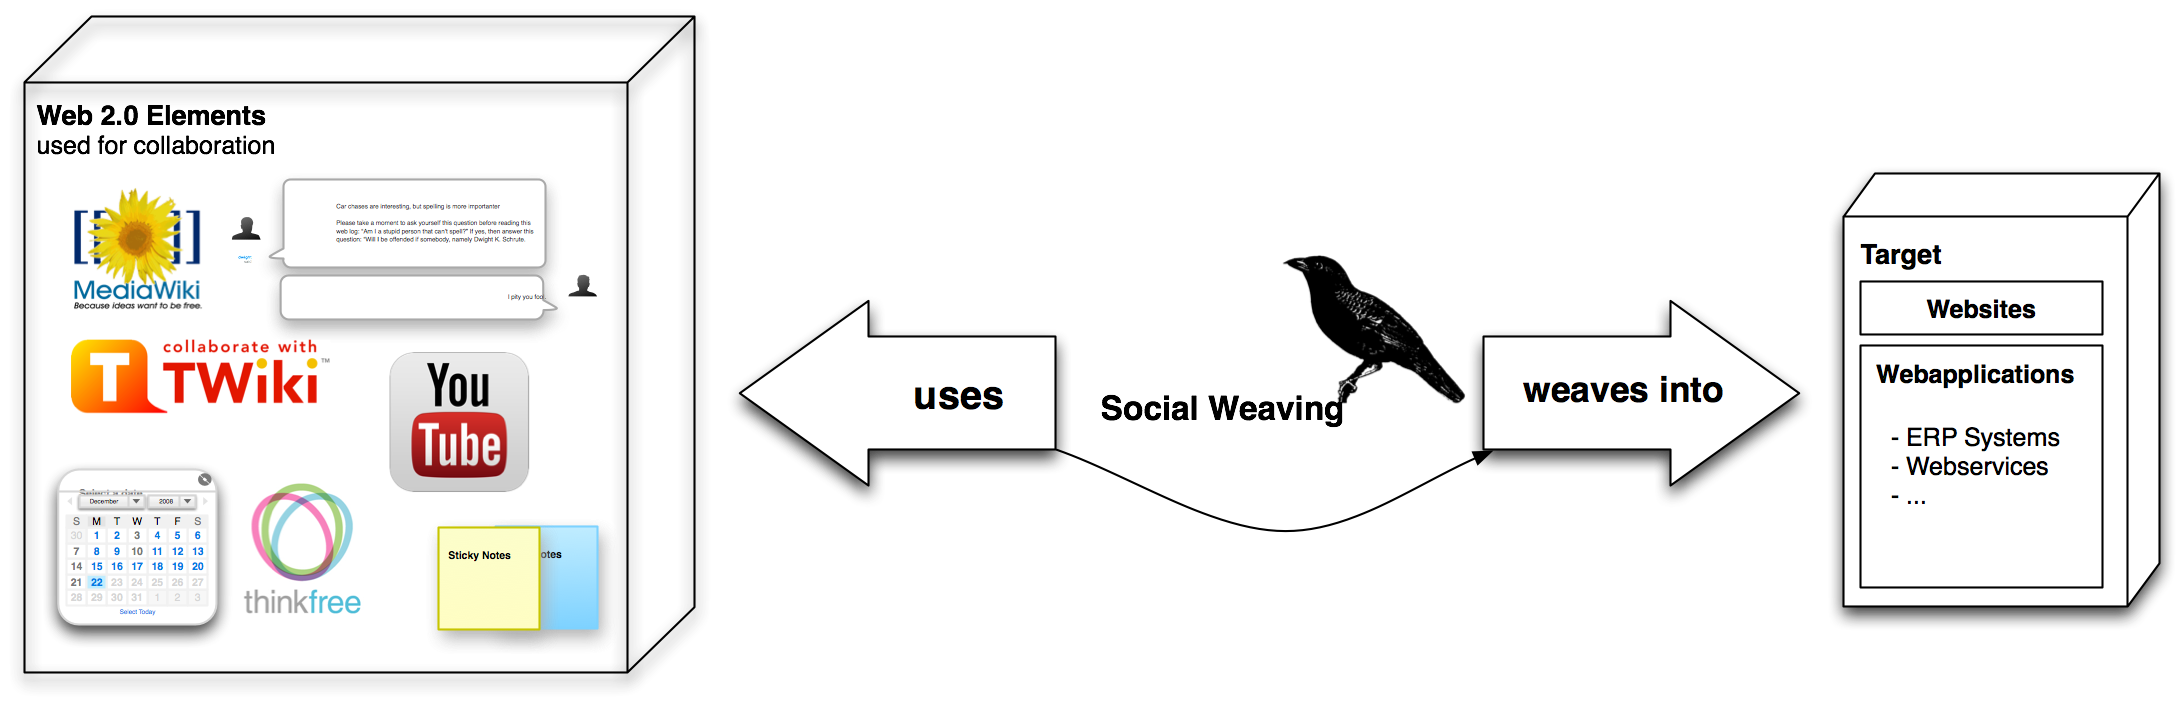
\includegraphics[width=13cm]{images/idead-social-weaving.png}
		\caption{Basic idea of Social Weaving}
		\label{idead-social-weaving}
\end{figure} 


So in combination we want the possibility to create some form of communication functionality - directly related to the button. And which is visible to a group of users for optionally unlimited amount of time.

Well if the web application would have an implemented comment box beneath the button, that would solve the problem. But that  solution brings another bunch of disadvantages. It would require to modify the web application that includes this functionality. And we cannot add comment boxes, links, ... to any element just as precautionary measure. This attempt of solution is not an option. 

What if we would have the opportunity to inject social elements directly into our web application without the need to modify it. Basically web applications run in a browser and what is displayed can be modified locally. And that is what we do. We weave social elements into the browser view and synchronize it for different user sessions. This way we reach exactly the functionality we need to solve our problem without touching the web application. We call this process Social Weaving. 

Even though Social Weaving overcomes the above mentioned problems - it confronts us with new types of pretty unpleaseant difficulties. Different browser types, unreliable web development styles, complex web technologies, etc. are examples for hurdles that Social Weaving has to deal with. 

This thesis will show what is possible with Social Weaving and where its boundaries are. 

In the following we are first going to discuss the idea of Social Weaving based on  an abstract requirements analysis of a prototype. What functionality does it need to achieve the goals we mentioned above and what are the difficulties? In the second part we are going down on a concrete level where we take the theory from the first part into action and actually explain the architecture and implementation of the prototype, Social Weaver, in detail. 